\subsection{Entity-Relationship Schema}

\begin{figure}
    \centering
    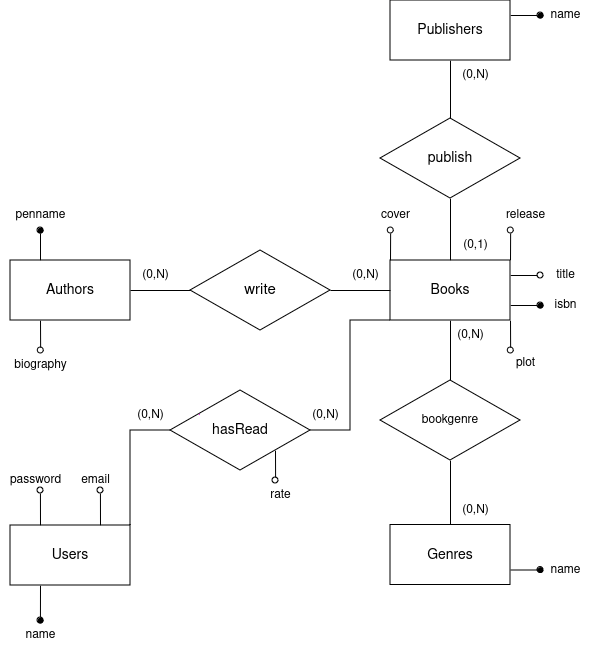
\includegraphics[width=0.85\linewidth]{DBbookrec4.png}
    \caption{ER schema of the database}
    \label{fig:enter-label}
\end{figure}

%Describe here your ER schema

The ER schema for the database is quite simple:
\begin{itemize}
    \item \textbf{Users}: this entity represent the users registered in the website, they are described by a \textit{name} (the application is not formal, so just the username should be enough) and by the login credentials \textit{email} and \textit{password}.
    \item \textbf{Books}: this entity contains all the main information about a book, like its \textit{title}, \textit{plot}, \textit{release} date and \textit{ISBN code}, in addition to its \textit{cover} image for aesthetic purpose in the website.
    \item \textbf{Authors}: here we have the various authors of the books present in the website, with information about them such as \textit{pen name} and \textit{biography}.
    \item \textbf{Publishers}: simple entity to store efficiently the publisher of books, with only the attribute \textit{name}.
    \item \textbf{Genres}: simple entity to store the genres of the books, described only by its \textit{name}.
\end{itemize}
For what concerns the relationships, we have:
\begin{itemize}
    \item \textbf{wrote}: this relationship connect one or more authors to one or more books; a book can have more than one author and an author, likely, wrote more than just one book.
    \item \textbf{hasRead}: this relationship connects users to books which they read and which they can rate on a scale from 1 to 5; it's a N:N relationship, since a user can read more than one book and books can be read by many users.
    \item \textbf{bookGenre}: this relationship connects books to their genres and it's N:N (a book can have more than one genre and vice versa)
    \item \textbf{publish}: this relationship connects books to their publishers; a book with a ISBN code can only be published by one publisher, so this is a 1:N relationship with books on the 1 side, while a publisher can have multiple books in its catalog.
\end{itemize}